\section{Convex sets and convex functions}

\begin{definition}[Convex Set]
	A set $\mathcal{C}$ is convex if and only if
	$\forall x,y \in \mathcal{C}$ and
	$\forall \theta \in [0,1]$: \quad
	$\theta x + (1-\theta)y \in \mathcal{C}$.
\end{definition}


\textbf{Examples of convex sets:}
\begin{itemize}
	\item
	      hyperplane $\{x \in \mathbb{R}^n \mid a\T x=b\}$
	\item
	      half-space $\{x \in \mathbb{R}^n \mid a\T x\le b\}$
	\item
	      polyhedron $\{x \in \mathbb{R}^n \mid Ax \preceq b ,\ Cx = d\}$

	      $A \in \mathbb{R}^{q\times n},\ C \in \mathbb{R}^{r\times n},\ b \in \mathbb{R}^{q},\ d\in \mathbb{R}^{r}$
	\item
	      ...more...

\end{itemize}

\subsection{Operations that preserve convexity (sets)}

\begin{itemize}
	\item \textbf{Intersection}
	      $\mathcal{C}_1, \mathcal{C}_2$ convex $\Rightarrow \mathcal{C}_1 \cap \mathcal{C}_2$ convex
	\item \textbf{Image under affine map}
	      $\mathcal{C} \subseteq  \mathbb{R}^{n}$ convex
	      $\Rightarrow \{Ax+b \mid x \in \mathcal{C} \}$ convex
	\item inverse image of an affine map:
	      ...
\end{itemize}

\subsection{Separating Hyperplane Theorem}

\begin{theorem}
	$\mathcal{C} \subseteq \mathbb{R}^{n}$ non-empty closed convex set, $y \notin \mathcal{C}$
	$\rightarrow \exists\ a \ne 0, b \in \mathbb{R}$
	s. t. $a\T x + b < a\T y + b,
		\forall x \in \mathcal{C}$
\end{theorem}

\begin{proof}
	\textbf{Claim}
	$\exists\ \hat{x} \in C$ s.t. $|\hat{x}-y|\leq |x-y|\quad \forall x \in \mathcal{C}$

	\textbf{Proof of claim}
	$|x-y|$ has bounded level sets,
	$\mathcal{C}$ is non-empty and closed
	$\Rightarrow \exists\ \hat{x} \in \underset{x \in \mathcal{C}}{\operatorname{argmin}}|x-y|$

	Hyperplane, we choose $a:=y-\hat{x}, b:=-a\T\hat{x} = -(y-\hat{x})\T\hat{x}$

	As a result, $a\T x + b = (y-\hat{x})\T (x-\hat{x})$
	and therefore $a\T y + b = |y-\hat{x})|^2 > 0$.
	The following claim shows that the hyperplane $a\T y + b$ seperates $\mathcal{C}$ and $y$.


	\textbf{Claim}
	$a\T y + b \le 0\quad \forall x \in \mathcal{C}$

	\textbf{Proof of claim}
	Assume not.
	$\rightarrow \exists\ x \in \mathcal{C}$ s.t.
	$(y-\hat{x})\T (x-\hat{x}) > 0$

	PARAMETRIZE $\theta$

	Contradiction $\hat{x}$ nearest point to $y$

	(Details in Lecture notes)
\end{proof}

\begin{corollary}
	A closed convex set $\mathcal{C} = \mathbb{R}^n$
	is the intersection of the closed half-spaces
	that contain $\mathcal{C}$.
\end{corollary}

\begin{proof}
	$\mathcal{S}$ intersection of closed half-spaces that contain $\mathcal{C}$

	1) $\mathcal{C} \subseteq \mathcal{S}: x \in \mathcal{C}$
	$\Rightarrow x$ is contained in every half-spaces that contains $\mathcal{C}$
	$\Rightarrow x$ is also contained in the intersections of half-spaces that contains $\mathcal{C}$
	$\Rightarrow x \in \mathcal{S}$

	2) $\mathcal{S} \subseteq \mathcal{C}:$
	Assume not
	$\rightarrow\ \exists\ \hat{x}\in \mathcal{S}$
	with $\hat{x}\notin \mathcal{C}$.
	By the Seperating Hyperplane Theorem there exists a hyperplane
	that seperates $\hat{x}$ from $\mathcal{C}$.
	That means there exists a closed half-space
	that contains $\mathcal{C}$ but not $\hat{x}$,
	hence $\hat{x}\notin \mathcal{C}$, contradiction.
\end{proof}

\subsection{Support function}

\textbf{Idea} represent any closed convex set by its supporting hyperplanes

Support Function: $\sigma_\mathcal{C}(a) = \underset{x \in \mathcal{C}}{\operatorname{sup}}a^Tx$

CALCULATION EXAMPLE

If we know the $\sigma_\mathcal{C}(a)$, we arrive at at

$$  \mathcal{C} = \bigcap_{a \in \mathbb{R}^n} \{x \in \mathbb{R}^n \mid a\T x - \sigma_c(a) \leq 0\}$$

$$   = \{x \in \mathbb{R}^n \mid \underset{a \in \mathbb{R}^{n}}{\operatorname{sup}}\ a\T x - \sigma_\mathcal{C}(a) \le 0\}$$

\begin{definition}
	A function $f : \mathbb{R}^n \rightarrow \mathbb{R}$
	is convex if and only if its epigraph is a convex set, where
	$$\operatorname{epi}(f):=\{(x,t)\in \mathbb{R}^{n+1} | f(x) \le t \}$$
\end{definition}

$\rightarrow$ this provides a link between convex sets and functions

\subsection{Operations that preserve convexity (functions)}

\begin{itemize}
	\item the pointwise maximum of convex functions is convex
	\item the sum of convex functions is convex
	\item $f(Ax+b)$ is convex if $f$ is convex
\end{itemize}

\subsubsection{How to check if f is convex?}

\begin{itemize}
	\item if $f: \mathbb{R}^n \rightarrow \mathbb{R}$ twice differentiable,
	      $\partial^2f/\partial x^2 \succeq 0\ \forall\ x \in \mathbb{R}^{n}$

	\item if $g: \mathbb{R} \rightarrow \mathbb{R}$ with $g(t)=f(x+tv)$
	      convex in $t\ \forall\ x,v \in \mathbb{R}^{n}$,
	      then $f$ is convex
	\item composition of simple convex function with convexity preserving operations
\end{itemize}

\textbf{Extended real numbers} $\bar{\mathbb{R}} = \mathbb{R} \cup \{+\infty, -\infty\}$


\textbf{Indicator function}
$\psi_\mathcal{C}(x) := \begin{cases} +\infty &\text{if } x \notin\mathcal{C} \ge 0 \\ 0 &\text{if } x \in\mathcal{C} \end{cases}$

$\rightarrow$ this provides another link between convex sets and functions

We can write
$\min_{x \in \mathcal{C}}f(x)$ as
$\min_{x \in \mathbb{R}^{n}}f(x) + \psi_\mathcal{C}(x)$

\begin{definition}[3]
	$f: \mathbb{R}^{n}\rightarrow\bar{\mathbb{R}}$ is called proper
	if $f$ is bounded below and
	if $\exists\ x \in \mathbb{R}^{n}$ s. t. $f(x)<\infty$
\end{definition}

\begin{definition}[Legendre Transformation]
	The conjugate function of $f: \mathbb{R}^{n}\rightarrow\bar{\mathbb{R}}$  is defined as
	$f^\star(y)=\underset{x \in \mathbb{R}^{n}}{\operatorname{sup}}y\T x-f(x)$
\end{definition}

IMAGE F-STAR

\subsection{Summary of Concepts}

% \begin{figure}[H]
% 	\centering
% 	% \includegraphics[width=\columnwidth]{images/X}
% 	\caption{cap}
% \end{figure}

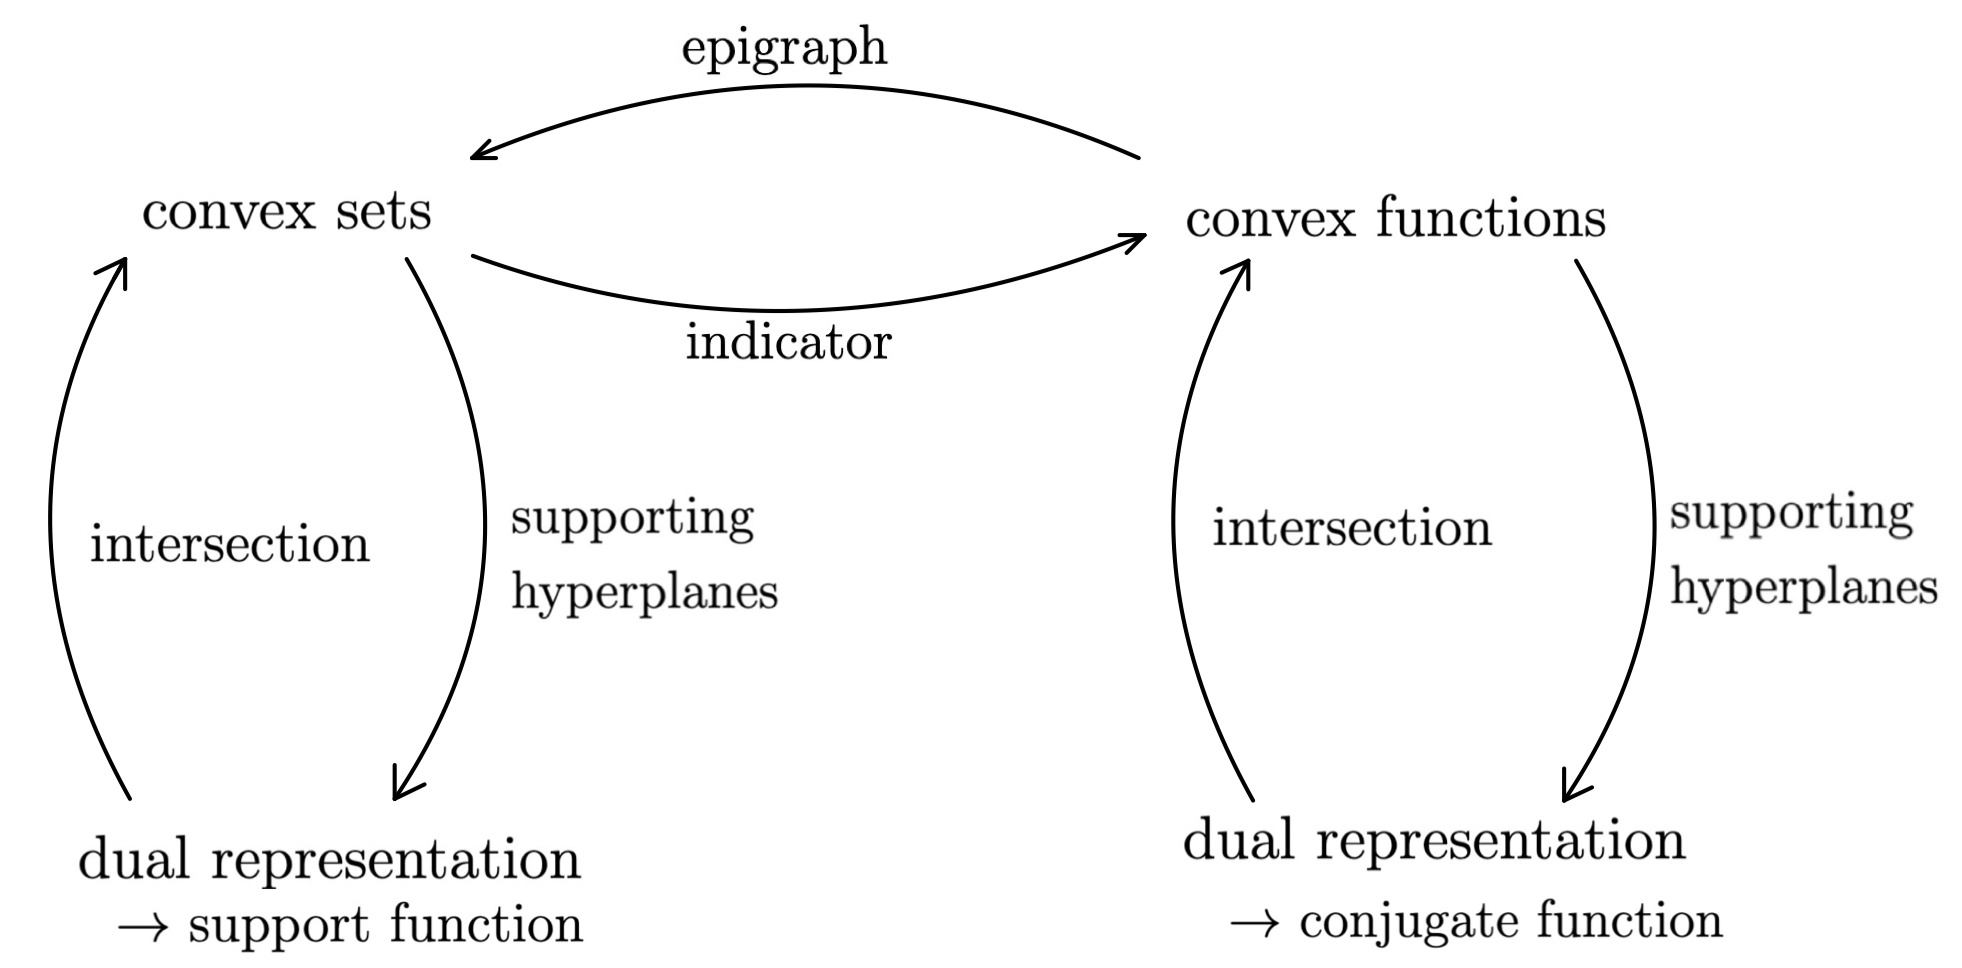
\includegraphics[width=\columnwidth]{images/summary_set_functions.png}

\begin{theorem}[THEOREM2?]

\end{theorem}
